\documentclass[12pt]{article}
\usepackage[backend=bibtex,style=numeric]{biblatex} 
\usepackage{graphicx}
\usepackage{hyperref}

\hypersetup{
    colorlinks=true,
    linkcolor=black,
    urlcolor=blue
}

\addbibresource{references.bib} 

\title{Report for the CPS Mid-Course Project}
\author{
    Andrea Auletta - 2107158 \\ \texttt{andrea.auletta@studenti.unipd.it} \and
    Niccolò Zenaro - 2125609 \\ \texttt{niccolo.zenaro@studenti.unipd.it}
}
\begin{document}

\maketitle
\newpage
\tableofcontents
\newpage

\section{Introduction and objectives}
In this report we will describe the work done for the mid-course project of the course 
Cyber-Physical Systems and IoT security. 
The paper to which we refer is \textbf{\cite{Cho2016} \citetitle{Cho2016}} where is explained 
the design of an algorithm: the CIDS (Clock-based Intrusion Detection System), that is able 
to detect different kinds of attack. In this paper is shown the functioning of three kinds 
of attack: the "Fabrication attack", the "Suspension attack" and the "Masquerade attack". 
What we tried to do was to implement the three attacks and the CIDS algorithm in a simulation 
environemnt using \textbf{ICSim}, instead of physically as shown in the paper.
\section{System setup}
We worked on a virtual machine with \textbf{LinuxMint22} as operating system.
The simulator used is \textbf{ICSim}. All the code is written in \textbf{Python} and can 
be found at the following link: \href{https://github.com/auli16/cpsProjectCANBus}{https://github.com/auli16/cpsProjectCANBus}.
We used the \textbf{can library} to create messages and to simulate the communication of the attackers with 
the ECUs.
The procedure to run the code is the following:
\begin{enumerate}
    \item In the directory where the simulator is located:
    \begin{verbatim}
    ./setup_vcan.sh    //set up a virtual can interface 
    ifconfig vcan0     //verify vcan0 interface is up
    ./icsim vcan0      //run the simulator
    ./controls vcan0   //control panel
    \end{verbatim}
    \item Run \textit{simulation.py} to create a dump of the CAN bus messages:
    \begin{enumerate}
        \item Select which attack to perform by changing the variable \textit{scriptAttack};
        \item Initially the script will run the periodic ECU and also the candump command
        will start;
        \item After 20 seconds will begin the attack;
        \item All the processes will be closed after 40 seconds after the beginning of the attack.
    \end{enumerate}
    
\end{enumerate}
\section{Experiments}
For each attack we are assuming that the attacker is already in the system and is able to send messages to 
several ECUs. To emulate a periodic ECU so that you can at least see something in the simulator we created 
the script \textit{periodicECU.py} where are sent messages every 2 seconds to open and close a certain number of 
doors of the car.  
\subsection{Fabrication attack}
In the Fabrication attack we are trying to inject messages into the CAN bus to make the system behave in a 
different way. Essentially, we created a message with the ID of the doors in a way that in the middle of 
those two seconds gap between legitimate messages we sent other commands to open and close the doors and 
causing it to function differently from normal behavior.
\subsection{Suspension attack}
In the Suspension attack we are trying to stop the receiving of messages sent by a legitimate ECU. We made 
a DoS like attack: we sent a big quantity of messages with the same ID of the doors into the CAN bus in order 
to lose the messages sent by it. Here we put a very small time sleep, precisely because the aim is to clog 
the network and not receive packets from legitimate ECUs. The result was that the doors were stuck in the same 
state.
\subsection{Masquerade attack}
In the Masquerade attack we are trying to send messages with the ID of the legitimate ECUs. The idea here 
is that we have to shield the fact that an ECU is compromised. After running the weak ECU script, the 
attacker will listen the CAN bus for 20 seconds, in this way it can calculate the period of the messages 
sent by the weak ECU and then it will send messages with the same ID and the same period. We decided to 
send a message to open different doors with respect to the ones opened by the weak ECU, and this can be 
seen at simulation time.
\subsection{CIDS algorithm}
CIDS is a new type of Intrusion Detection System (IDS) that is Clock-based. The algotithm measures and 
exploits the interval of periodic messages for fingerprinting ECUs. These fingerprints are then used for 
deriving a clock-behavioural scheme obtained by the Recursive Least Squares (RLS) algorithm. RLS is 
applied to timestamps and their offsets to derive covariance and skewness. Based on this scheme, 
CIDS uses the cumulative sum to detect shifts in the clock skew, in fact the intrusion is detected 
monitoring this parameter. We worked direcly on the dumps of the CAN bus messages obtained through 
the command \textit{candump}. In each dump file we used \textit{periodicECU.py} to send periodic 
messages from the ECU \textit{0x19B}
In the file \textit{cids.py} we implemented the algorithm, this is composed by several 
parts:
\begin{enumerate}
    \item Data preprocessing: we've taken the timestamps of the messages and we've inserted them 
    in a vocabulary in which you can access with the ID of the ECU;
    \item Offset calculation: the offset is given by the difference of the timestamps and the corresponding
    expected time (calculated with the period of the messages);
    \item Recursive square least algorithm: we've implemented the RLS algorithm to calculate the covariance 
    and the skew;
    \item CUSUM algorithm: we've implemented the CUSUM algorithm to detect the intrusion. 
\end{enumerate}
Given the ID in which we are interested, as return we will get an indication of whether the ECU is
compromised or not.
\section{Results and Discussion}
As said before we've implemented the three attacks and the CIDS algorithm in a simulation environment.
We've taken different dumps of the CAN bus messages and we've analyzed them with the CIDS algorithm. 
The parameters which we've finetuned are the following:
\begin{itemize}
    \item \textbf{threshold}: for the CUSUM algorithm is set to 5, it is used to 
    understand given a certain value if there was an intrusion or not;
    \item \textbf{kappa}: is a value which also is used to make the system more or less sensitive to the offsets;
    \item \textbf{window\_size}: Effectively we are trying to emulate a CIDS algorithm in real time, 
    so we have to considere a window of messages to analyze up to a ceratin moment. We've set this value to 
    20 in a way to consider 20 * i offset at a time, where i is the number of the iteration 
    of the CUSUM algorithm.
\end{itemize}
We've got 4 dump files of the CAN bus messages:
\begin{itemize}
    \item \textit{dump\_noAttack.log}: this is the dump of the CAN bus messages without any attack. The algorithm 
    didn't detect any intrusion for the ID of interest (419 = 0x19B).
    \begin{center}
        \vspace{-1cm}
        \hspace*{-2cm}
        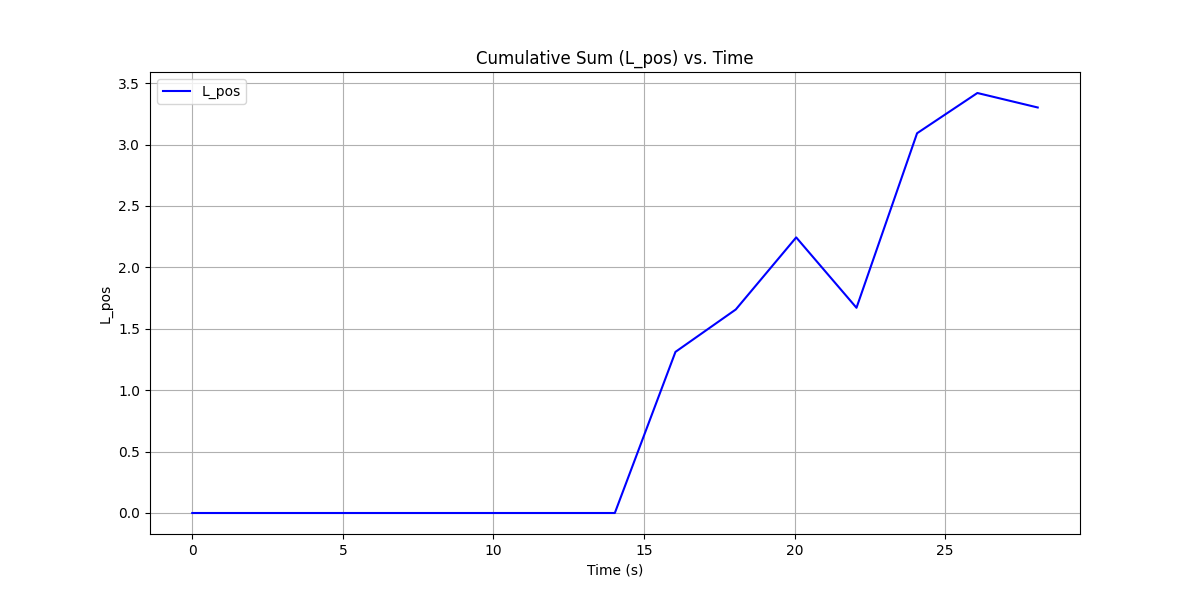
\includegraphics[scale=0.5]{img/LposNoAttack.png}
    \end{center}
    Since $L_{pos}$ does not exceeds the given threshold, 
    we can conclude that in this dump we have no attacks for this ECU, confirming what we expected;
    \item \textit{dump\_fabr.log}: this is the dump of the CAN bus messages with the Fabrication attack. The ID 
    of interest is detected as compromised (419 = 0x19B);
    \begin{center}
        \vspace{-1cm}
        \hspace*{-2cm}
        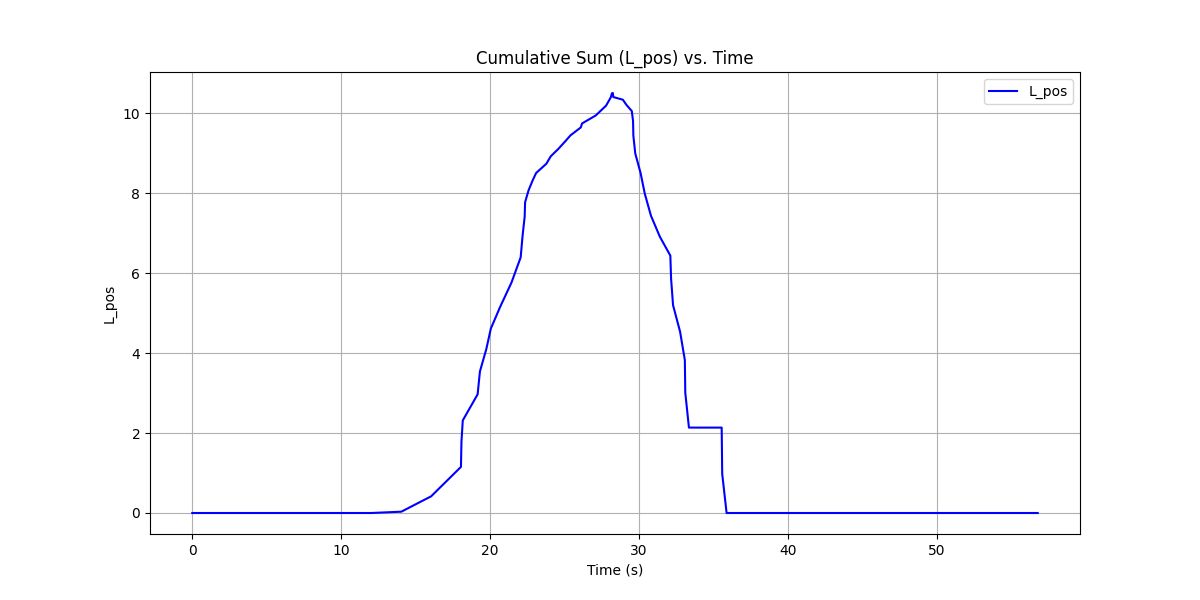
\includegraphics[scale=0.5]{img/LposFabr.png}
    \end{center}
    In the image above $L_{pos}$ exceeds the threshold after 20 seconds, therefore we have a compromised ECU. 
    The shape of the curve characterizes a Fabrication Attack;
    \item \textit{dump\_susp.log}: this is the dump of the CAN bus messages with the Suspension 
    attack. The ID of interest is detected as compromised (411 = 0x19B);
    \begin{center}
        \vspace{-0.5cm}
        \hspace*{-2cm}
        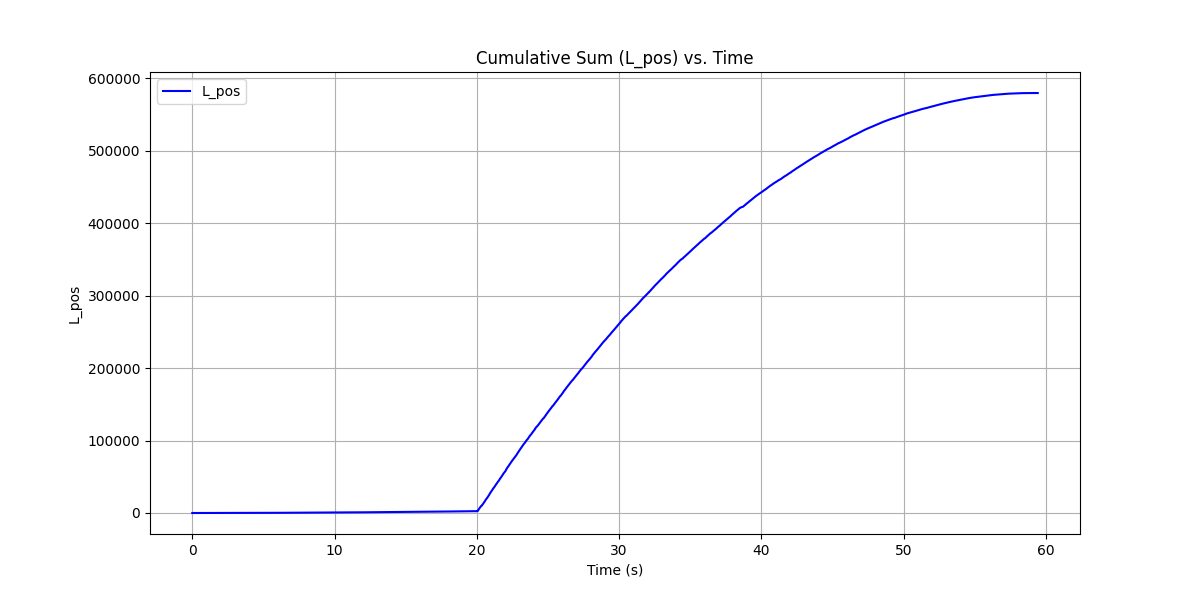
\includegraphics[scale=0.5]{img/LposSusp.png}
    \end{center}
    The value of $L_{pos}$ starts to increase after 20 seconds and it follows a logarithmic behavior. The values
    reached by $L_{pos}$ are really high due to the fact we are sending a lot of messages with the same ID.
    CIDS is detecting an intrusion since the values are above the threshold;
    \item \textit{dump\_masq.log}: this is the dump of the CAN bus messages with the Masquerade attack. 
    The ID of interest is detected as compromised (419 = 0x19B), in this case with a lower value 
    of L with respect to the Fabrication attack. 
    \begin{center}
        \vspace{-1cm}
        \hspace*{-2cm}
        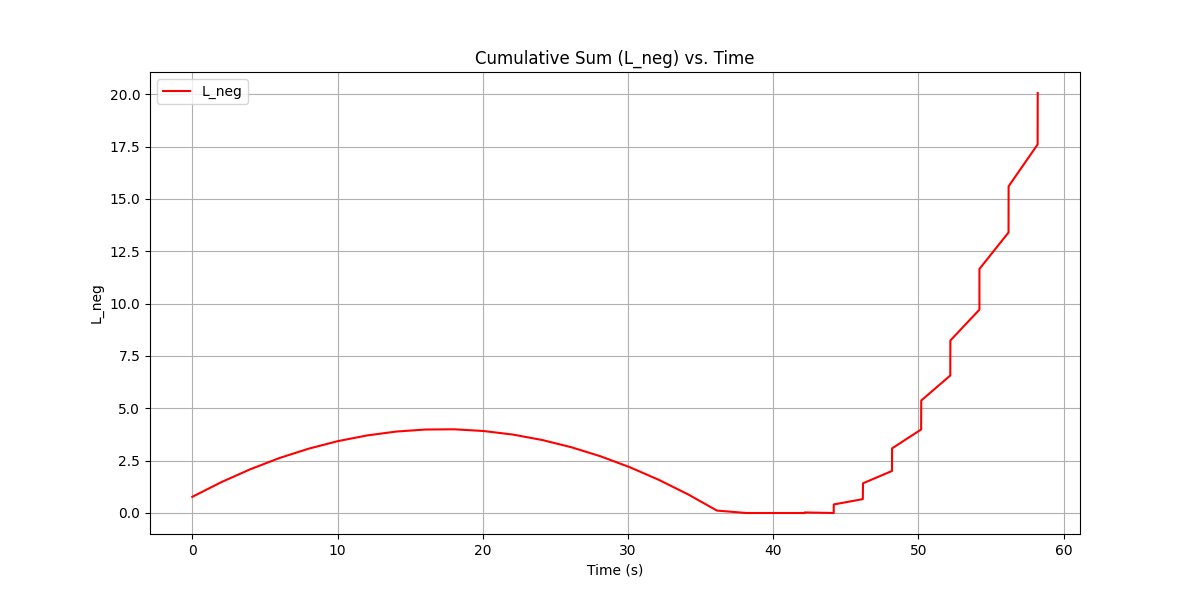
\includegraphics[scale=0.5]{img/LnegMasq.png}
    \end{center}
    The initial curve is under the threshold, and the values start to grow after 40 seconds because of the implementation of the attack.
    After that time CIDS is able to detect the variations in $L_{neg}$.
\end{itemize}
In conclusion we can say that we had similar results and plots to the ones shown in the reference paper. 

\printbibliography 

\end{document}
